\documentclass[../main.tex]{subfile}
\graphicspath{{\subfix{../images}}}
\begin{document}

我们将物体检测的独立组件统一到一个神经网络中。我们的网络使用来自整个图像的特征来预测每个边界框。它还同时预测图像的所有类别的所有边界框。这意味着我们的网络对完整图像和图像中的所有物体进行全局推理。YOLO设计支持端到端训练和实时速度,同时保持高平均精度。

我们的系统将输入图像划分为$ S \times S $网格。如果物体的中心落入网格单元中,则该网格单元负责检测该物体。

每个网格单元预测$ B $个边界框和这些框的置信度。这些置信度反映了模型对框包含物体的信心程度,以及它认为盒子预测的准确度。形式上,我们将置信度定义为$\text{Pr}\left(\text{Object}\right) \ast \text{IOU}^\text{truth}_\text{pred}$。如果该单元格中不存在物体,则置信度分数应为零。否则,我们希望置信度得分等于预测框和ground truth之间的交集(IOU)。

每个边界框由 5 个预测组成:$x,y,w,h $和置信度。 $(x,y)$ 坐标表示相对于网格单元边界的框中心。宽度和高度是相对于整个图像预测的。最后,置信度预测表示预测框和任何ground truth框之间的IOU。

每个网格单元还预测$ C $个条件类概率,$\text{Pr}\left( \text{Class}_i \vert  \text{Object} \right)$。这些概率以网格单元包含物体的为条件。我们只为每个网格单元预测一组类概率,而不管框$ B $的数量。

在测试时,我们将条件类概率和单个框置信度预测相乘,
\begin{equation}
    \text{Pr}\left( \text{Class}_i \vert  \text{Object} \right) \ast \text{Pr}\left(\text{Object}\right) \ast \text{IOU}^\text{truth}_\text{pred} = \text{Pr}\left( \text{Class}_i \right) \ast \text{IOU}^\text{truth}_\text{pred}
\end{equation}
这为我们提供了每个框特定类的置信度分数。这些分数编码了该类出现在框中的概率以及预测的框与物体的匹配程度。

\begin{figure}[htb]
    \centering
    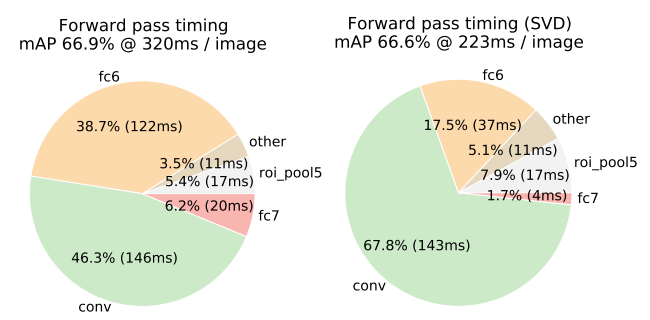
\includegraphics[width=\textwidth]{fig2.png}
    \caption{\textbf{模型。}我们的系统将检测建模为一个回归问题。它将图片划分为$S\times S$个网格,并为每个网格预测$B$个边界框、这些边界框的置信度和$C$个类别概率。这些预测被编码为一个$S\times S \times \left( B \ast 5 + c \right)$的张量。}
    \label{fig:fig2}
\end{figure}

为了在 PASCAL VOC 上评估 YOLO,我们使用 $S = 7$,$B = 2$。PASCAL VOC 有 20 个标记类别,因此$ C = 20$。我们的最终预测是一个 $7 \times 7 \times 30$ 张量。

\subsection{网络设计}

我们将此模型实现为卷积神经网络,并在 PASCAL VOC 检测数据集\cite{pascal}上对其进行评估。网络的初始卷积层从图像中提取特征,而全连接层预测输出概率和坐标。

我们的网络架构受到用于图像分类的GoogLeNet模型的启发\cite{googlenet}。我们的网络有24个卷积层,后跟 2 个全连接层。我们不使用 GoogLeNet 使用的inception模块,而是简单地使用$ 1 \times 1 $缩减层和$ 3 \times 3 $卷积层,类似于 Lin 等人\cite{nin}。完整的网络如图\ref{fig:fig3}所示。

\begin{figure}[htb]
    \centering
    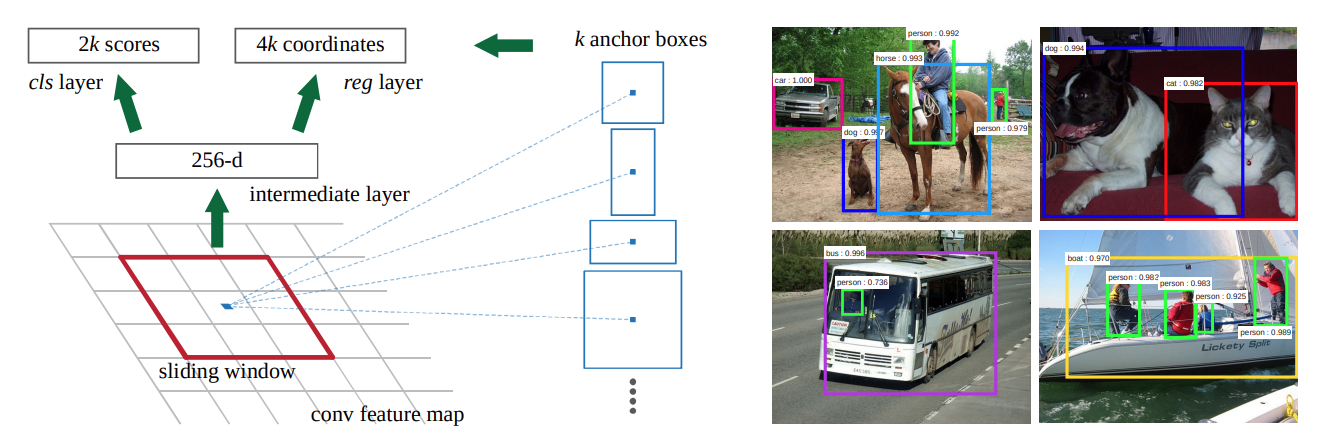
\includegraphics[width=\textwidth]{fig3.png}
    \caption{\textbf{网络结构。}我们的检测网络有 24 个卷积层,后跟 2 个全连接层。 交替的$ 1 \times 1 $卷积层减少了前一层的特征空间。 我们在 ImageNet 分类任务上以一半的分辨率($224 \times 224 $输入图像)预训练卷积层,然后将分辨率提高一倍以进行检测。}
    \label{fig:fig3}
\end{figure}

我们还训练了一个快速版本的 YOLO,旨在突破快速目标检测的边界。 Fast YOLO 使用较少卷积层(9 个而不是 24 个)并在这些层中使用较少的卷积核。除了网络的大小之外,YOLO 和 Fast YOLO 的所有训练和测试参数都是相同的。

我们网络的最终输出是$ 7 \times 7 \times 30 $的预测张量。

\subsection{训练}

我们在 ImageNet 1000 类竞赛数据集 [30] 上预训练我们的卷积层。对于预训练,我们使用图\ref{fig:fig3}中的前 20 个卷积层,然后是平均池化层和全连接层。我们对该网络进行了大约一周的训练,并在 ImageNet 2012 验证集上实现了 88\% 的单次裁剪 top-5 准确率,与 Caffe 的 Model Zoo [24] 中的 GoogLeNet 模型相当。我们使用darknet框架进行所有训练和推理 [26]。

然后我们转换模型以执行检测。Ren等人表明将卷积层和连接层添加到预训练网络可以提高性能 [29]。按照他们的例子,我们添加了具有随机初始化权重的四个卷积层和两个全连接层。检测通常需要细粒度的视觉信息,因此我们将网络的输入分辨率从$ 224 × 224 $增加到$ 448 × 448$。

我们的最后一层预测类别概率和边界框坐标。我们通过图像的宽度和高度对边界框的宽度和高度进行归一化,使它们落在 0 和 1 之间。我们将边界框的$ x $和$ y $坐标参数化为特定网格单元位置的偏移量,因此它们也被限制在 0 和 1 之间.

我们对最后一层使用线性激活函数,所有其他层使用以下leaky校正线性激活:
\begin{equation}
    \phi\left(x\right) = \left\{
    \begin{aligned}
         & x,    & \text{if }x > 0  \\
         & 0.1x, & \text{otherwise}
    \end{aligned}
    \right.
\end{equation}

我们针对模型输出中的平方和误差进行了优化。我们使用平方和误差是因为它很容易优化,但是它并不完全符合我们最大化平均精度的目标。它将定位误差与分类误差同等加权,这可能并不理想。此外,在每个图像中,许多网格单元不包含任何物体。这会将这些单元格的“置信度”分数推向零,通常会压倒包含物体的单元格的梯度。这可能会导致模型不稳定,从而导致训练早期出现发散。

为了解决这个问题,我们增加了边界框坐标预测的损失,并减少了不包含物体的框的置信度预测的损失。我们使用两个参数$ \lambda_\text{coord} $和$ \lambda_\text{noobj} $来实现这一点。我们设置$ \lambda_\text{coord} = 5 $和$ \lambda_\text{noobj} = 0.5$。

平方和误差也同样加权大框和小框的错误。我们的误差度量应该反映大盒子中的小偏差比小盒子中的小偏差重要性小。为了部分解决这个问题,我们预测边界框宽度和高度的平方根,而不是直接预测宽度和高度。

YOLO 为每个网格单元预测多个边界框。在训练时,对于每个物体,我们只希望一个边界框预测器对它负责。我们根据哪个预测与ground truth具有最高的 IOU 来指定哪一个预测器为此ground truth“负责”。这导致边界框预测器之间的专业化。每个预测器在预测特定大小、长宽比或物体类别方面都变得更好,从而提高了整体召回率。

在训练期间,我们优化了以下多部分损失函数:
\begin{equation}
    \begin{aligned}
         &   & \lambda_\text{coord}\sum_{i=0}^{S^2}\sum_{j=0}^{B}\mathbbm{1}_{ij}^\text{obj}\left[ \left(x_i - \hat{x}_i\right)^2 + \left(y_i - \hat{y}_i\right)^2 \right]                             \\
         & + & \lambda_\text{coord}\sum_{i=0}^{S^2}\sum_{j=0}^{B}\mathbbm{1}_{ij}^\text{obj}\left[ \left(\sqrt{w_i} - \sqrt{\hat{w}_i}\right)^2 + \left(\sqrt{h_i} - \sqrt{\hat{h}_i}\right)^2 \right] \\
         & + & \sum_{i=0}^{S^2}\sum_{j=0}^{B}\mathbbm{1}_{ij}^\text{obj}\left(C_i - \hat{C}_i\right)^2                                                                                                 \\
         & + & \lambda_\text{noobj}\mathbbm{1}_{ij}^\text{noobj}\left(C_i - \hat{C}_i\right)^2                                                                                                         \\
         & + & \sum_{i=0}^{S^2}\mathbbm{1}_i^\text{obj}\left(p_i\left(c\right) - \hat{p}_i\left(c\right)\right)^2
    \end{aligned}
\end{equation}
其中$\mathbbm{1}_i^\text{obj}$表示物体是否在单元$i$出现,$\mathbbm{1}_{ij}^\text{obj}$表示单元$i$的第$j$个边界框预测器对这个检测“负责”。

请注意,仅当该网格单元中存在物体时(因此是前面讨论的条件类概率),损失函数才会惩罚分类错误。仅当该预测器对ground truth框“负​​责”(即具有该网格单元中任何预测器的最高 IOU)时,它才会惩罚边界框坐标错误。

我们在来自 PASCAL VOC 2007 和 2012 的训练和验证数据集上训练网络约 135 个epoch。在 2012 测试时,我们在训练时还使用了 VOC 2007 的测试数据。在整个训练过程中,我们使用 64 的批量大小、0.9 的动量和 0.0005 的衰减。

我们的学习率计划如下:对于第一个epoch,我们慢慢地将学习率从$10^{-3} $提高到$ 10^{-2}$。如果我们以高学习率开始,我们的模型通常会因梯度不稳定而发散。我们继续用$ 10^{-2} $训练 75 个epoch,然后用$ 10^{-3} $训练 30 个epoch,最后用$ 10^{-4} $训练 30 个epoch。

为了避免过拟合,我们使用 dropout 和广泛的数据增强。在第一个连接层之后具有 rate = .5 的 dropout 层来防止层之间的协同适应 [18]。对于数据增强,我们引入了最多原始图像大小 20\% 的随机缩放和平移。我们还在 HSV 色彩空间中随机调整图像的曝光和饱和度,最高达 1.5。

\subsection{推理}

就像在训练中一样,预测测试图像的检测只需要一次网络评估。 在 PASCAL VOC 上,网络预测每个图像的 98 个边界框和每个框的类别概率。 YOLO 在测试时非常快,因为它只需要一次网络评估,这与基于分类器的方法不同。

网格设计在边界框预测中强制执行空间多样性。 通常很清楚一个物体属于哪个网格单元,并且网络只为每个物体预测一个框。 但是,一些大型物体或靠近多个单元格边界的物体可以被多个单元格很好地定位。 非最大抑制可用于修复这些重复检测。 虽然对 R-CNN 或 DPM 的性能并不重要,但非最大抑制在 mAP 中增加了 2-3\%。

\subsection{YOLO的局限}

YOLO 对边界框预测施加了很强的空间约束,因为每个网格单元只预测两个框并且只能有一个类。 这种空间约束限制了我们的模型可以预测的附近物体的数量。 我们的模型在处理成群出现的小物体时遇到了困难,例如成群的鸟。

由于我们的模型学习从数据中预测边界框,因此它很难泛化到具有新的或不寻常的长宽比或配置的物体。 我们的模型还使用相对粗略的特征来预测边界框,因为我们的架构包含对输入图像的多个下采样层。

最后,当我们训练近似检测性能的损失函数时,我们的损失函数将小边界框与大边界框的错误处理相同。 大框的小错误通常是良性的,但小框的小错误对 IOU 的影响要大得多。 我们的主要错误来源是不正确的定位。

\end{document}